\documentclass[tikz,border=5pt]{standalone}
\usepackage{tikz}
\usetikzlibrary{arrows.meta, positioning, fit}

\begin{document}

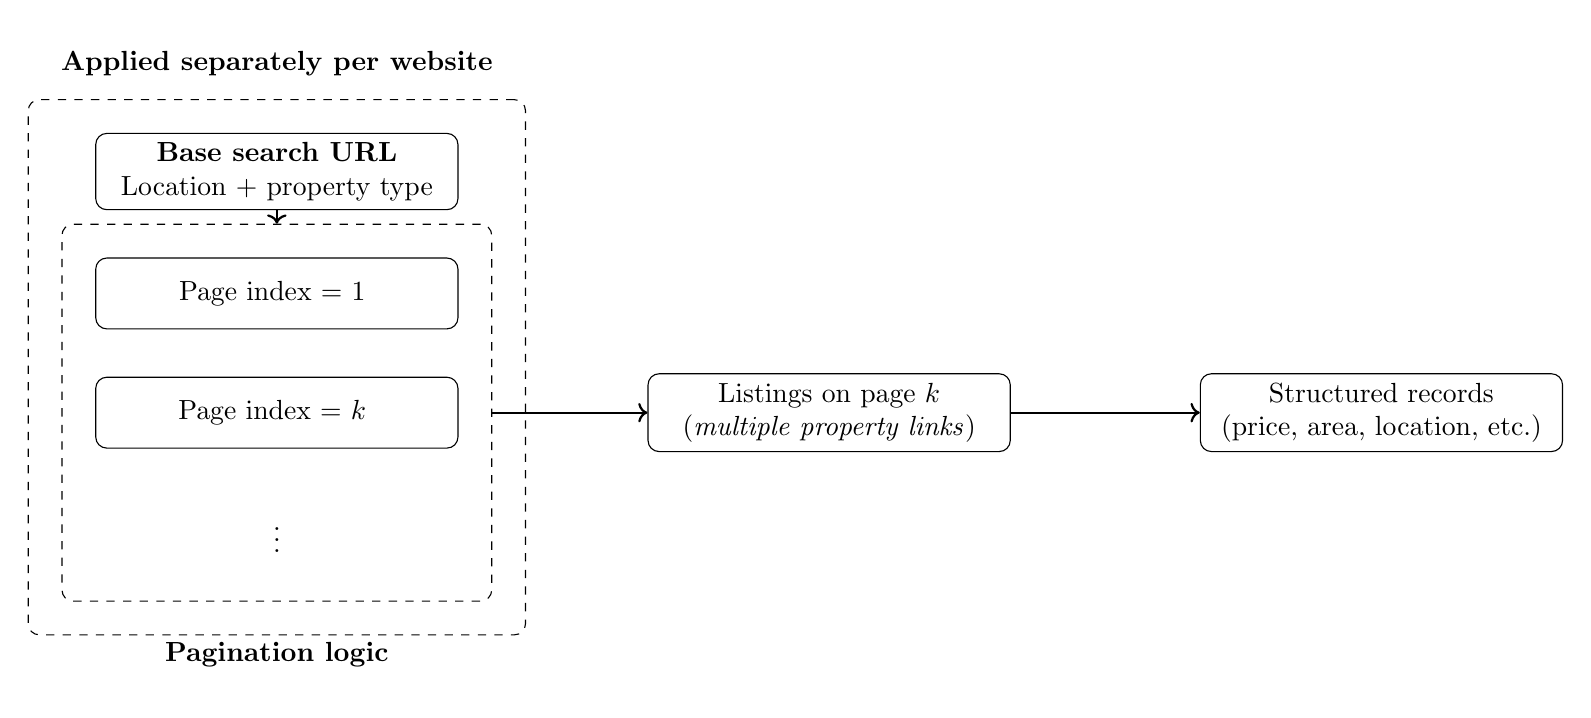
\begin{tikzpicture}[
    every node/.style={
        draw,
        rounded corners,
        align=center,
        minimum width=4.6cm,
        minimum height=9mm
    },
    arrow/.style={->, thick},
    node distance=10mm
]

% ------------------------
% Base URL
% ------------------------
\node (base) {
\textbf{Base search URL}\\
Location + property type
};

% ------------------------
% Pagination nodes
% ------------------------
\begin{scope}[node distance=6mm]
\node (page1) [below=of base] {
Page index = 1
};

\node (pagek) [below=of page1] {
Page index = $k$
};

\node[draw=none, below=of pagek] (dots) {$\vdots$};
\end{scope}
% ------------------------
% Pagination logic (dashed box)
% ------------------------
\node[
    draw,
    dashed,
    rounded corners,
    fit=(page1)(pagek)(dots),
    inner sep=12pt,
    label={[yshift=-6pt]below:{\textbf{Pagination logic}}}
] (pagebox) {};

% ------------------------
% Listings extraction
% ------------------------
\node (listings) [right=24mm of pagek] {
Listings on page $k$\\
(\textit{multiple property links})
};

% ------------------------
% Record construction
% ------------------------
\node (records) [right=24mm of listings] {
Structured records\\
(price, area, location, etc.)
};

% ------------------------
% Arrows (KEY FIX)
% ------------------------
\draw[arrow] (base.south) -- (pagebox.north);
\draw[arrow] (pagebox.east) -- (listings.west);
\draw[arrow] (listings.east) -- (records.west);

% ------------------------
% Applied separately per website (outer dashed box)
% ------------------------
\node[
    draw,
    dashed,
    rounded corners,
    fit=(base)(pagebox),
    inner sep=12pt,
    label=above:{\textbf{Applied separately per website}}
] {};

\end{tikzpicture}

\end{document}
